\documentclass[letterpaper]{article}
\usepackage[utf8]{inputenc}
\usepackage{array}
\usepackage{wrapfig}
\usepackage{multirow}
\usepackage{tabu}
\usepackage{graphicx}
\usepackage{verbatim}

\title{Software Requirements Specification} 

\author{
	Vincent Boivin, ID 27419694 \and
	Kisife Giles, ID 40001926 \and
	Marc-Antoine Jette-Leger, ID 27895038 \and
	Jean-Loup Johnston, ID 40006259 \and
	Fabian Vergara, ID 40006706 \and
	Michael Xu, ID 27206356
}


\begin{document}
	
\maketitle

   \vspace*{\stretch{1.0}}
   \begin{center}
      \Large\textbf{Software Requirements Specification}\\
      \large\textit{Prepared by Group PA-PJ}\\
   \end{center}
   \vspace*{\stretch{2.0}}
   
   


\tableofcontents

\newpage

\section{Revision History}

	\paragraph{Tuesday February 6th, 2018 Version 1.0}  
	
	\paragraph{Tuesday February 7th, 2018 Version 1.1}  
	Reworked context, added Business rules, Non-functional requirements
	
	\paragraph{Tuesday February 9th, 2018 Version 1.2}  
	Described Use Case 3, added Domain Model, added the domain model entries to the glossary, formatted tables and lists
	
\newpage

\newpage

\section{Project Description}

    \subsection{Purpose}
		Our team has been given a mandate to design and implement a money budgeting application for use by the clients of our customer. The application aims to provide a representation of a user's current spending based on type and to offer him/her ways in which that spending can be changed. The purpose of this document is to provide the Software Requirement Specification (SRS) report for the the said application. The purpose of it is to give a high level overview and a full description of the functional and nonfunctional requirements of the system. It will also cover the system design and implementation constraints, and different external interfaces with which the system shall interface.
		
	\subsection{Introduction}
	
		Currently, many users have trouble discerning the way in which they spend their money unless they track it themselves, however, that task is arduous and time consuming. In order to offer customers with a clear representation of their finances, companies have developed complicated software to solve this task, however, often times, users hesitate to use it due to the aforementioned complexity. As a solution, we have been tasked with presenting customers with a simple, yet efficient and intuitive application.
	
	\subsection{Context}
	
		In the context of our application, the main way users will be able to interact with our application will be mainly through a desktop application. The application will use user provided user information (bank statement) in order to provide an assessment of the current spending.
	
	\subsection{Business goals}
	
		The primary business goal is to make our customers save more and to make them adopt our software applications, which will allow us to provide a better service as a more well rounded financial company. This in turn allows us to increase efficiency (needs less employees to serve customers on the same topic), increase our market share, as we did not have this service beforehand which will in turn increase our profit margin because we have access to more customers than before.
	
	\subsection{Scope}
	
		The MyMoneyApp software is a financial management application, developed in Java as a standalone desktop application targeting young consumers. This system’s aim is to help users to make wise and accurate decisions when they have a target amount of savings they want to have for a month. It performs this operation by first getting the user’s bank statement, then displaying them on-screen to differentiate what amount of money has went into what type of service, and to then be able to change those amounts in the coming months. The main qualities of MyMoneyApp, is that it is easy-of-use, user-friendly and efficient, which will allow the purchasing company to satisfy its customers’ needs. All in all, this software will help the company to hold its market leader position in the financial domain.
	
	\subsection{Domain model}
	
		\begin{center}
			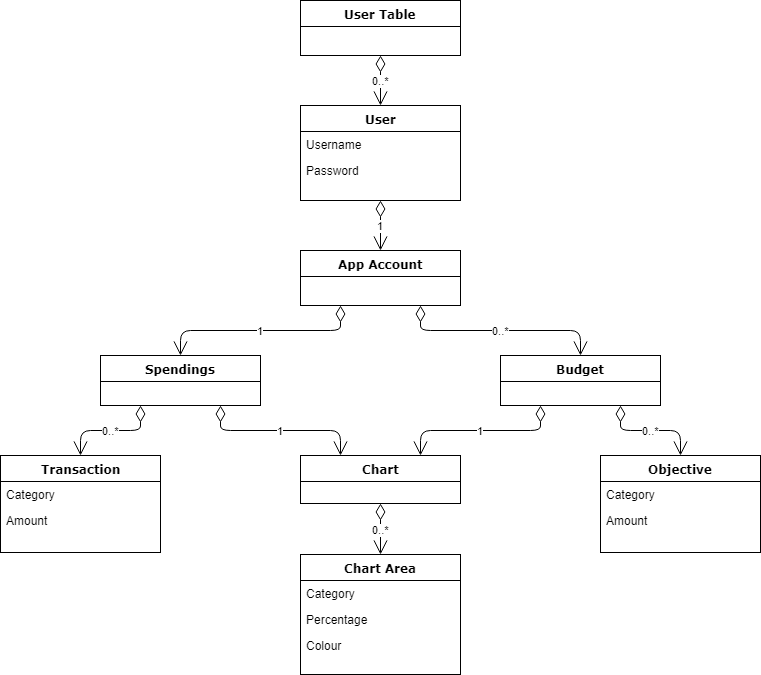
\includegraphics[height=10cm]{DomainModel}
		\end{center}
		
	\subsection{Class Diagram}
	
		\begin{center}
			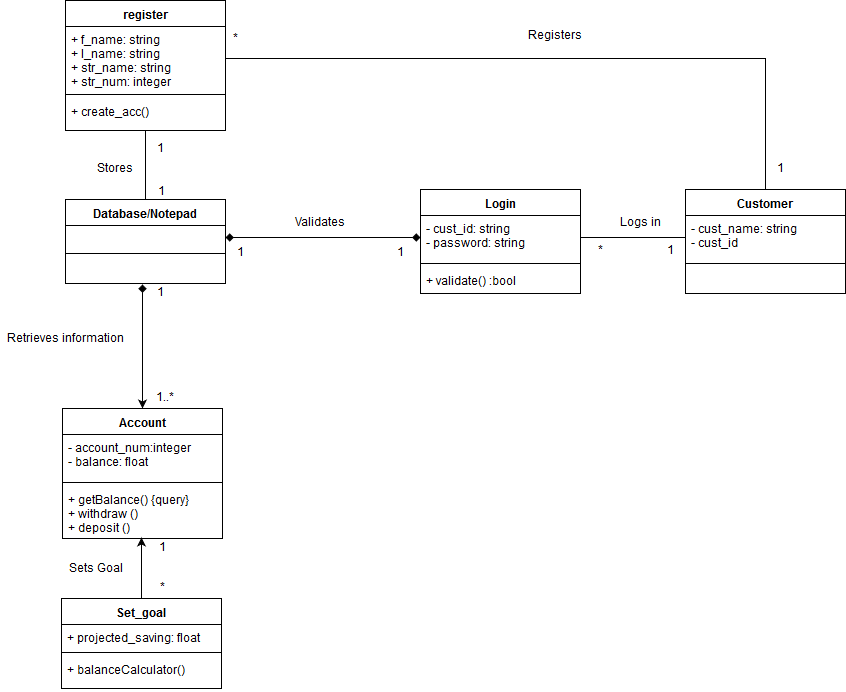
\includegraphics[height=10cm]{Classdiagram}
		\end{center}
		
	\subsection{Actors}
	
		This document is intended to be read by:
		
		\begin{itemize}
			
			\item Users of the software: this document allows them to have a more complete idea about the system and its functionality.
			
			\item Team developers: they can use this document as a primary resource for all subsequent project development phases (design, coding, testing and maintenance phases).
			
			\item Testers: To be able to test the system in accordance to the specified requirements.
			
			\item CEO of the company that has hired us: this document will allow them to deeper understand and have a more comprehensive idea about the requirements of the project.
			
		\end{itemize}

\section{Functional requirements}

	\subsection{Overview}
	
		This section includes all the details regarding the use cases and features afforded to the user of the MyMoney application. Those features include creating and logging into an account, accessing various information about the transactions made with a bank account, and creating, inspecting and deleting budgetary goals to be stored in a list.
	
	\subsection{Use cases}
	
		\subsubsection{Create user accounts}
		
        \begin{center}
        	\begin{tabular}{ | m{3.5cm} | m{7.5cm}| } 
	            \hline
	            \textbf{Action} & Account management \\ 
	            \hline
	            \textbf{Case ID} & 1.1 \\ 
	            \hline
	            \textbf{Summary} & User provides the necessary information for the creation of an account. \\
	            \hline
	            \textbf{Scope} & Budget management application \\ 
	            \hline
	            \textbf{Trigger} & Registration button \\
	            \hline
	            \textbf{Precondition} & None \\ 
	            \hline
	            \textbf{Postcondition} & Account is created \\ 
	            \hline
	            \textbf{Primary Actor} & User \\ 
	            \hline
	            \textbf{Secondary Actor} & Filesystem \\ 
	            \hline
        	\end{tabular}
        
        	\vspace{2mm}
        
			\begin{tabular}{ | m{3.5cm} | m{7.5cm}| } 
				\hline
	            \textbf{Main Scenario-Step} & \textbf{Action} \\ 
	            \hline
	            1 & User Clicks on Register. \\ 
	            \hline
	            2 & User enters a username, password, and password confirmation, and click “Register Account” button. \\ 
	            \hline
	            3 & System verifies if the username is already taken. \\ 
	            \hline
	            4 & System gets login credentials from File System. \\ 
	            \hline
	            5 & System verifies in login file if the password and password confirmation are the same. \\ 
	            \hline
	            6 & System creates account object. \\ 
	            \hline
	            7 & System saves the username and password combination to the database/textpad. \\
	            \hline
	            8 & System displays login menu, with account creation confirmation, and asks user to login. \\ 
	            \hline
	            9 & System goes idle. \\ 
	            \hline
        	\end{tabular}
        \end{center}
        
        \subsubsection{Access user accounts}
		
        \begin{center}
	        \begin{tabular}{ | m{3.5cm} | m{7.5cm}| } 
	            \hline
	            \textbf{Action} & Account management \\ 
	            \hline
	            \textbf{Case ID} & 1.2 \\ 
	            \hline
	            \textbf{Summary} & User provides the necessary information to login. \\
	            \hline
	            \textbf{Scope} & Budget management application \\ 
	            \hline
	            \textbf{Trigger} & Login button \\
	            \hline
	            \textbf{Precondition} & Have a registered account \\ 
	            \hline
	            \textbf{Postcondition} & Account is accessed \\ 
	            \hline
	            \textbf{Primary Actor} & User \\ 
	            \hline
	            \textbf{Secondary Actor} & Filesystem \\ 
	            \hline
	        \end{tabular}
        
        	\vspace{2mm}
        
			\begin{tabular}{ | m{3.5cm} | m{7.5cm}| } 
				\hline
	            \textbf{Main Scenario-Step} & \textbf{Action} \\ 
	            \hline
	            1 & User inputs username and password. \\ 
	            \hline
	            2 & User clicks on the “login” button. \\ 
	            \hline
	            3 & System verifies if the username, password pair exists. \\ 
	            \hline
	            4 & System displays the user's transaction logs. \\ 
	            \hline
	            5 & System goes idle. \\ 
	            \hline
	        \end{tabular}
        \end{center}

		\subsubsection{Load and display transactions data}
		
		\begin{center}
	        \begin{tabular}{ | m{3.5cm} | m{7.5cm}| } 
	            \hline
	            \textbf{Action} & Load and display transaction data \\ 
	            \hline
	            \textbf{Case ID} & 2 \\ 
	            \hline
	            \textbf{Summary} & User provides the the number of his credit card number for the reviewing of his spending. \\
	            \hline
	            \textbf{Scope} & Budget management application \\ 
	            \hline
	            \textbf{Trigger} & Get my info button \\
	            \hline
	            \textbf{Precondition} & To be logged in as a user \\ 
	            \hline
	            \textbf{Post condition} & Transaction data is displayed \\ 
	            \hline
	            \textbf{Primary Actor} & User \\ 
	            \hline
	            \textbf{Secondary Actor} & Filesystem \\ 
	            \hline
	        \end{tabular}
        
        	\vspace{2mm}
        
           	\begin{tabular}{ | m{3.5cm} | m{7.5cm}| } 
           		\hline
	            \textbf{Main Scenario-Step} & \textbf{Action} \\ 
	            \hline
	            1 & User Enters his credit card number. \\ 
	            \hline
	            2 & User clicks on the get transaction data button. \\ 
	            \hline
	            3 & System pulls the information from the textpad/database. \\ 
	            \hline
	            4 & Transaction data is displayed on the screen. \\ 
	            \hline
	            5 & System goes idle. \\ 
	            \hline
	        \end{tabular}
        \end{center}
        
		\subsubsection{Create and visualize budget}
		
		\begin{center}
			\begin{tabular}{ | m{3.5cm} | m{7.5cm}| } 
				\hline
				\textbf{Action} & Account customization \\ 
				\hline
				\textbf{Case ID} & 3 \\ 
				\hline
				\textbf{Summary} & The user is able to create a budget and visualize it with a chart \\
				\hline
				\textbf{Scope} & Budget management application \\ 
				\hline
				\textbf{Trigger} & Budget button \\
				\hline
				\textbf{Precondition} & To be logged in as a user \\ 
				\hline
				\textbf{Postcondition} & Budget information displayed and editable, chart is accessible \\ 
				\hline
				\textbf{Primary Actor} & User \\ 
				\hline
			\end{tabular}
		
			\vspace{2mm}
		
			\begin{tabular}{ | m{3.5cm} | m{7.5cm}| } 
				\hline
				\textbf{Main Scenario-Step} & \textbf{Action} \\ 
				\hline
				1 & User clicks the Budget button \\ 
				\hline
				2 & User chooses a category \\ 
				\hline
				3 & User enters an amount \\ 
				\hline
				4 & User clicks the Add to budget button \\ 
				\hline
				5 & User's budget is updated in real time \\ 
				\hline
				6 & User clicks Create chart button \\ 
				\hline
				7 & User's budget is instantly computed and illustrated by a chart in a new window \\ 
				\hline
				8 & User clicks the Reset budget button \\ 
				\hline
				9 & User's budget values are all set to 0 \\
				\hline
				10 & User's budget is updated in real time \\  
				\hline
			\end{tabular}
		\end{center}
	
	\subsection{Business Rules}
	
		\begin{itemize}
			
			\item The customer must not be able to alter his balance that he entered (read only)
			
			\item The customer must have a credit card with a balance on it (textpad in this case)
			
		\end{itemize}
	
\section{Non-functional requirements}

	\begin{itemize}
		
		\item The login information (password/username) is encrypted 
		
		\item The application is intuitive to use and requires no computer knowledge
		
	\end{itemize}

\section{Design Constraints}

	The programming language used in this software is Java. The main feature is giving a clear representation of the user’s spending over the course of a bank statement. The representation will take the form of graphs and charts defining where their money went. Users can only view their past data and cannot alter it. The maintenance and feature upgrades are handled by us, the developers of MyMoneyApp.

\section{Glossary}

	\paragraph{User table}
	
		The user table is the collection of registered users, along with their login information
	
	\paragraph{User}
	
		A user is the virtual representation of a person using the application
	
	\paragraph{App account}
	
		An account is the model used by the application to store and use a user's information and interact with all the different features present in the application
	
	\paragraph{Spending}
	
		A user's spending is the agglomeration of every transaction done and entered by the user
	
	\paragraph{Budget}
	
		A user's budget is the collection of the user's projected spending
	
	\paragraph{Chart}
	
		A chart is the graphic illustration of the user's spending or budget information
	
	\paragraph{Chart area}
	
		A chart area represents a category of the user's projected or actual spending, represented by a percentage of the total spending or budget and unique color in the chart, indicating which category the area relates to
		
	\paragraph{Transaction}
	
		A transaction summarizes a positive or negative money transaction made by the user in real life and is composed of the amount of money exchanged during the transaction and the category which the transaction relates to (e.g. food, home, transportation, salary, ...)
		
	\paragraph{Objective}
		
		An objective is an entry reflecting a projected amount spent in a given category. It is composed of a category and an amount. These values are used by the system to produce a budget for the user, illustrated by a chart if the user so chooses)
	
	\begin{comment}
	\paragraph{Transaction}
	
	A transaction summarizes a positive or negative money transaction made by the user in real life and is composed of the amount of money exchanged during the transaction, the date when the transaction was made, the business the transaction was completed with, and the category which the transaction relate to (e.g. food, home, transportation, salary, ...)
	
	\paragraph{Budgetary objective}
	
		A budgetary objective represents a goal that the user wishes to aim towards in term of money saving. An objective tracks how much money was spent on what category or categories of goods and services in a set amount of time and compares it with a set goal. A budgetary objective is considered a success if the amount of money spent in the tracked amount of time on the tracked objective is smaller than the set goal. It is tagged as “In progress” if the period of time tracked includes the current date. It is considered a failure otherwise.
	\end{comment}

\section{References}

    Larman, C. (2016). Applying UML and patterns. Chennai: Pearson.\\
    Sommerville, I. and Sommerville, I. (2006). Software engineering 7.5. Harlow: Addison-Wesley.\\

	
\end{document}
